\documentclass[a4paper,12pt]{article}
\usepackage{cmap}
\usepackage[utf8]{inputenc}
\usepackage[warn]{mathtext}
\usepackage{epsf,amsmath,amsfonts,amssymb,amsbsy}
\usepackage[mathscr]{eucal}
\usepackage[english, russian]{babel}
\usepackage[left=2cm,right=2cm,top=2cm,bottom=2cm]{geometry}
\usepackage{graphicx}
\usepackage{indentfirst}
\graphicspath{{Sharik_Diffuzia_picture/}}
\DeclareGraphicsExtensions{.pdf,.png,.jpg}
\usepackage{pgfplots}
\usepackage{icomma}
\usepackage{wrapfig}	
\author{Мещеряков Павел Б02-920}
\title{Лабораторная работа }
\begin{document}
		\maketitle
	\begin{center}
		{\Large Определение коэфициента диффузии гелия через резиновую оболочку воздушного шарика}
	\end{center}
	\paragraph{Цель работы:} Знакомство с явлениями переноса. Определение коэффициента диффузии гелия через резиновую оболочку резинового шарика. 
\paragraph{В работе используются:}  Два одинаковых резиновых шарика шарообразной формы, один из которых накачан гелием, весы (точность $0.01 \; г$), секундомер, груз известной массы, нитка, ножницы.
 
\section{Теоретическое введение}

Воздушный шарик, накачанный гелием, со временем достаточно быстро сдувается. Это связано с диффузией гелия через резиновую оболочку шарика. Плотность потока гелия 
$ j$ (число молекул, проникающих через единичную площадку резины в единицу времени) определяется законом Фика:
\begin{equation}
j=D\frac {\Delta n }{\delta}
\end{equation}
где $D$ - коэффициент диффузии гелия через резину, $\delta$ - толщина резиновой оболочки накаченного шарика, $\Delta n =n-n_0$ - разность концентраций гелия внутри $n$ и вне шарика $n_0$.
За время $t$ через всю поверхность резиновой оболочки шарика $S$ в атмосферу выйдет:

\begin{equation}
\Delta N=jSt=\frac{DSnt}{\delta}=\frac{DSNt}{\delta V}
\end{equation}
молекул гелия (внутри шарика концентрация $n = \frac{N}{V}$, вне шарика концентрацию гелия считаем равной нулю $n_0=0$). (В приведённой формуле $S$ считается константой).
Пренебрегая утечкой газа через узел, а также проникновением молекул воздуха внутрь шарика и, т.е., предполагая, что оболочка шарика проницаема только для гелия, получим, что относительное изменение величины подъёмной силы шарика $F_п=(\rho_0-\rho_{He})Vg$ за время $t$ равно:
\begin{equation}
\frac {\Delta F_п}{ F_п} =\frac {\Delta V}{ V}=-\frac {\Delta N} {N}=-\frac{DSt}{\delta V}
\end{equation}
откуда:
\begin{equation}
\Delta F_п=-\frac{DS F_п t}{\delta V}=-\frac{DS (\rho_0-\rho_{He})gt}{\delta }
\end{equation}
Эта формула даёт закон изменения подъёмной силы с течением времени:
\begin{equation}
F_п(t)=F_0-\frac{DS (\rho_0-\rho_{He})gt}{\delta }
\end{equation}
В приведённых выше формулах $\rho_0$ - плотность окружающего шарик воздуха, $ \rho_{He}$ - плотность гелия в шарике. При этом мы считали, что давление гелия внутри шарика незначительно превосходит атмосферное (реально, для шаров шарообразной формы давление в шарике превосходит атмосферное на $\approx 5\%$ из-за давления Пуассона, связанного с кривизной тела).
\section{Методика измерений}

	
	
	\begin{wrapfigure}[18]{r}{0.15\linewidth} 
		\vspace{-4.5ex}
		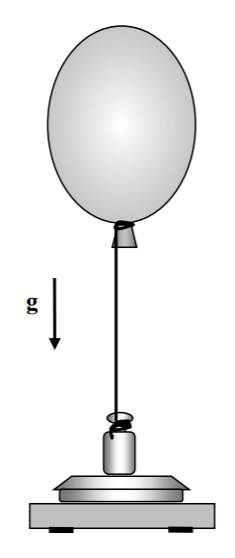
\includegraphics[width=4cm]{sharik}
		\label{fig5}
	\end{wrapfigure}

Привяжем к нити гелиевого шарика груз и положим груз на весы как показано на рисунке. Сила тяжести груза превышает подъёмную силу шарика. Сила, действующая на платформу весов, равна:
\begin{equation}
F=m_{гр}g-F_п
\end{equation}
Поскольку с течением времени подъёмная сила уменьшается линейно,
то показания весов, начиная с некоторого начального значения $m_0$, увеличиваются по линейному закону:
\begin{equation}
m(t)=m_0+\beta t
\end{equation}Таким образом, коэффициент диффузии $D$ можно определить по значению углового коэффициенту $\beta$ графика экспериментальной зависимости $m(t)$ по формуле:
\begin{equation}
D=\frac{\beta \delta } { S(\rho_0-\rho_{He})}
\end{equation}
\section{Выполнение и обработка}
Площадь  поверхности шара оценим, приближая её полусферой и конусом: $S = \frac{\pi d^2 + \pi ld}{2},$ где $d$ — диаметр обхвата шарика, $l$— длина ребра. Результаты измерений:
$$ \pi d = 75.0 \pm 0.2 \, см,  \; l = 17.5 \pm 0.2\,  см.$$
Погрешность $S$ оценивается по формуле:
$$\sigma_S = S \cdot \sqrt{\Big(\frac{2\sigma_{d}}{d}\Big)^2+\Big(\frac{\sigma_{d}}{d}\Big)^2+\Big(\frac{\sigma_{l}}{l}\Big)^2 + \Big(\frac{\sigma_{т}}{S}\Big)^2},$$
где $\frac{\sigma_{т}}{S}$ я оцениваю в $10\%$, как ошибку которую даёт сама формула. В итоге $$S = (1.55 \pm 0.16) \cdot 10^{-1}\; м^2.$$ 

Для оценки толщины резины $\delta$ измеряем массу растягивающейся части (т.е отрезаем хвостик второго шарика) шарика $m=2.30 \; г$ и поделив на площадь и плотность шарика $\rho = 1.05 \; \frac{г}{см^3}$, погрешность оценивается по следующей формуле:
$$\sigma_{\delta} = \delta \sqrt{\Big(\frac{\sigma_{m}}{m}\Big)^2+ \Big(\frac{\sigma_{S}}{S}\Big)^2}.$$ 
В результате получим $$\delta = (1.41 \pm 0.14) \cdot 10^{-2} \; мм.$$
Плотность воздуха  $\rho_0=1.16\,  \frac{кг}{м^3}$, плотность гелия, $ \rho_{He}=0.16 \,  \frac{кг}{м^3}$.
\\\\
Результаты измерений показаний весов от времени приведены в таблице:

% 	\begin{center}
%		\begin{tabular}{|l|l|l|l|l|l|l|l|l|l|}
%  			\hline
%  			$m, г$   & 6.28 & 6.31 & 6.34 & 6.35 & 6.38 & 6.38 & 6.39 & 6.40 & 6.44 \\ \hline
%  		$	t, мин$ & 0    & 2    & 4    & 6    & 8    & 10   & 12   & 15   & 20   \\ \hline
%  			$m, г $ & 6.48 & 6.52 & 6.55 & 6.59 & 6.62 & 6.64 & 6.67 & 6.69 & 6.70 \\ \hline
%  		$	t, мин$ & 25   & 30   & 35   & 40   & 45   & 50   & 55   & 60   & 65   \\ \hline
%  		\end{tabular}
%  	\end{center}

  	  	\begin{center}
  		\begin{tabular}{|l|l|l|l|l|l|l|l|l|l|}
  			\hline
  			$m, г$   & 7.16 & 7.18 & 7.20 & 7.21 & 7.22 & 7.24 & 7.25 & 7.28 & 7.31 \\ \hline
  			$	t, мин$ & 0    & 2    & 4    & 6    & 8    & 10   & 12   & 15   & 20   \\ \hline
  			$m, г $ & 7.34 & 7.37 & 7.40 & 7.44 & 7.46 & 7.49 & 7.52 & 7.53 & 7.54 \\ \hline
  			$	t, мин$ & 25   & 30   & 35   & 40   & 45   & 50   & 55   & 60   & 65   \\ \hline
  		\end{tabular}
  	\end{center}
  	
  	Построим график зависимости $m(t)$ по точкам из таблицы. И с помощью мнк (предварительно отбросив 2 последние, которые явно выбиваются из линейной зависимости) определим параметры наилучшей прямой.
  	
%  \begin{center}
%\
%  		\begin{tikzpicture}[scale=1.5]
%  		\begin{axis}[
%  		axis lines = left,
%  		legend style={at={(1,0.3)}},
%  		xlabel = {$	t, мин$},
%  		ylabel = {$m, г $
%  		},
%  		xmin=0, xmax=70,
%  		ymin=6.20, ymax=6.8,
% 		ymajorgrids = true,
%  		xmajorgrids = true,
% 		grid = both,
%  		minor tick num = 4
% 		]
%  		\addplot+[only marks ] plot[error bars/.cd, y dir=both, y %explicit]
%  		coordinates {
  			
%  			(0,6.27) +- (0,0.01)
%  			(2,6.31) +- (0,0.01)
%  			(4,6.34) +- (0,0.01)
%  			(6,6.35) +- (0,0.01)
%  	  		(8,6.38) +- (0,0.01)
%  	  		(10,6.38) +- (0,0.01)
%  	  		(12,6.39) +- (0,0.01)
%  	  		(15,6.40) +- (0,0.01)
%  	  		(20,6.44) +- (0,0.01)
%  	  		(25,6.48) +- (0,0.01)
%  	  		(35,6.55) +- (0,0.01)
%  	  		(40,6.59) +- (0,0.01)
%  	  		(45,6.62) +- (0,0.01)
%  	  		(50,6.64) +- (0,0.01)
%  	  		(55,6.67) +- (0,0.01)
%  	  		(60,6.69) +- (0,0.01)
%  	  		(65,6.70) +- (0,0.01)
%	  		
% 		};
%			\addplot[red,domain=0:65]{0.0065*x + 6.3103};
%			\addplot[black,dashed,domain=0:65]{0.0075*x+6.26};
%			\addplot[black,dashed,domain=0:65]{0.0055*x+6.32};		
% 	
%  		\end{axis}
% 		\end{tikzpicture}	
%\end{center}

  \begin{center}
	\
	\begin{tikzpicture}[scale=1.5]
	\begin{axis}[
	axis lines = left,
	legend style={at={(1,0.3)}},
	xlabel = {$	t, мин$},
	ylabel = {$m, г $
	},
	xmin=0, xmax=70,
	ymin=7.10, ymax=7.6,
	ymajorgrids = true,
	xmajorgrids = true,
	grid = both,
	minor tick num = 4
	]
	\addplot+[only marks ] plot[error bars/.cd, y dir=both, y explicit]
	coordinates {

		
		(0,7.16) +- (0,0.01)
		(2,7.18) +- (0,0.01)
		(4,7.20) +- (0,0.01)
		(6,7.21) +- (0,0.01)
		(8,7.22) +- (0,0.01)
		(10,7.242) +- (0,0.01)
		(12,7.254) +- (0,0.01)
		(15,7.28) +- (0,0.01)
		(20,7.31) +- (0,0.01)
		(25,7.34) +- (0,0.01)
		(30,7.37) +- (0,0.01)
		(35,7.40) +- (0,0.01)
		(40,7.44) +- (0,0.01)
		(45,7.46) +- (0,0.01)
		(50,7.49) +- (0,0.01)
		(55,7.52) +- (0,0.01)
		(60,7.53) +- (0,0.01)
		(65,7.54) +- (0,0.01)
	};
	\addplot[red,domain=0:65]{0.00624*x + 7.176};
	%\addplot[black,dashed,domain=0:65]{0.0075*x+6.26};
	%\addplot[black,dashed,domain=0:65]{0.0055*x+6.32};
	
	
	\end{axis}
	\end{tikzpicture}	
\end{center}
Соответственно наклон прямой принимает следующее значение:
$$\beta = 10.4\cdot10^{-5} \;  \frac{г}{с}.$$
%$$\beta _{min}= 10,8\cdot10^{-5}\, г/с$$
%$$\beta_{max} = 11,7\cdot10^{-5}\, г/с$$
Погрешность коэффициента наклона находится из мнк:
$$\sigma_{\beta} = 0.4 \cdot 10^{-5} \; \frac{г}{с}$$
Погрешность $D$ можно оценить с помощью следующей формулы:
$$\sigma_D = D \cdot \sqrt{\Big(\frac{\sigma_{\beta}}{\beta}\Big)^2 + \Big(\frac{\sigma_{\delta}}{\delta}\Big)^2 + \Big(\frac{\sigma_{S}}{S}\Big)^2 }$$
%$$\frac{\Delta D} {D} = \frac {\beta_{max}-\beta_{min}} {2\beta}$$
Искомый коэффициент:
$$D = (0.95\pm0.15)\cdot10^{-7}\, \frac{см^2}{с}$$
Чтобы убедиться в том, что в шарик не попадает воздух, достаточно оценить объём шарика в конце эксперимента. Если воздух не проникал в шарик в ходе эксперимента, то подъёмная сила, вычисленная по формуле для силы Архимеда (в предположении, что в шарике гелий) и измеренная экспериментально, должны быть равны. Объём шарика рассчитаем, разбив его на полусферу и конус:
\begin{equation}
V=\frac{\pi d^2(d+\sqrt{l^2-{\frac d 2}^2})} {12}
\end{equation}

Учитывая предыдущие значения (шарик за время опыта сдулся не значительно), а также вычисляя по теореме Пифагора высоту конуса, находим $V=42.5\cdot10^2\, см^3$. Таким образом теоретическое значение подъёмной силы $$f_т = (\rho_{0} - \rho_{He})V = 4.25 \; г$$
Величину подъёмной силы измерить просто — достаточно придержать шарик, чтобы измерить массу груза. Она равна $10.00 \; г$. Масса пустого шарика — $3.00 \; г$. Тогда подъемная сила в конце эксперимента (через $1 \; час \;10 \; мин$) равна $5.46 \; г$. С достаточной степенью точности можно считать, что шарик по-прежнему заполнен только гелием.

\section{Выводы}
Получен экспериментально коэффициент диффузии гелия $D = (0.95\pm0.15)\cdot10^{-7}\, \frac{cм^2}{с}$
(теоретический коэффициент диффузии $D_{He-O_2}=0.68\cdot10^{-7}\,\frac{см^2}{c}$).
Отклонение в $\approx40\%$ связано прежде всего с приближенной оценкой формы шара. Вероятно, диффузия не равномерна из-за разной концентрации гелия в разных участках шарика, так же не исключено, что могли (иногда) возникать воздушные потоки, мешающие точным измерениям массы.\\
Экспериментально проверено то, что в пределах погрешности (выше упомянутой) шарик остается полностью заполнен гелием.
%
%\newpage
%\section{Контрольные вопросы}
%begin{enumerate}
%	\item$$\textbf{j}=-D \nabla n,$$  где $\nabla n \equiv \left ( \frac{\partial n}{\partial x},\frac{\partial n}{\partial y},\frac{\partial n}{\partial z}\right)$ градиент концентрации $n$,\\ $\textbf{j}$ поток частиц на соответствующую ось 
%\\
%\item$$D=\frac {1}{3}\overline{v}  \lambda$$
%$$\overline{v}=\sqrt{\frac {8RT}{\pi \mu}} -  средняя\: %скорость\: молекул$$
%$$\lambda=\frac {1} {\sqrt 2 \sigma n} - длина\: свободного\: %пробега\: молекул \; одного \; сорта$$
%Подставляя значения нормальных условий и характеристики гелия %получим
%$$D=0,83\cdot10^{-7}\,\frac{см^2}{c}.$$
%\item Воспользуемся законом Фика
%$$\frac {N} {St} = -D\frac 1 V \frac {dN} {dx} $$
%т.к $\frac{V}{S} = x$, то проинтегрировав это уравнение %получим
%$$D=\frac{x^2}{2t}=4,7\cdot10^{-8}\, \frac{cм^2}{с}.$$
%\item Воспользуемся прошлой формулой, так как процессы и %условия идентичны
%$$x=\sqrt{2Dt}=2,5\,см.$$
%\item $\mu = 0,5$ для резины означает, то что ее обьем %сохраняется, а нам это важно для проверки заполненности %шарика гелием.
%\end{enumerate}

\end{document}
